% !TeX program = xelatex
\documentclass[12pt]{article}
\usepackage[UTF8,fontset=none]{ctex}
\setCJKmainfont{Noto Serif CJK SC}
\usepackage{amsmath,amssymb}
\usepackage{geometry}
\geometry{a4paper,margin=1in}
\usepackage{graphicx}
\usepackage{float}
\newcommand{\unit}[1]{\,\mathrm{#1}}
\title{自动控制原理I实验一报告}
\author{Zhefeng Lin}
\date{}
\begin{document}
\maketitle
\section{实验目的与装置}
掌握编码器读取、电压输出和转速滤波方法；建立电机一阶转速模型及二阶位置闭环模型；比较仿真与实际系统的动态、稳态性能，分析比例增益对阶跃响应的影响。

实验采用QUBE-Servo系列旋转伺服装置，通过MATLAB/Simulink搭建模型，使用QUARC进行实时控制。模拟电压由HIL Write Analog输出，电机转角由编码器读取。编码器每转对应2048个计数，计数值$N$与转角的关系为
\begin{equation}
 \theta=\frac{2\pi}{2048}N.
\end{equation}
转角微分后经低通滤波得到转速估计，采用的滤波环节为
\begin{equation}
 G_f(s)=\frac{50}{s+50},\qquad
 \widehat\Omega(s)=\frac{50s}{s+50}\Theta(s).
\end{equation}

\section{理论建模}
\subsection{电压至转速的一阶模型}
电枢回路与机械运动方程分别为
\begin{align}
 V_m&=R_m i_m+L_m\frac{\mathrm di_m}{\mathrm dt}+k_m\omega_m,\\
 J_{\mathrm{eq}}\frac{\mathrm d\omega_m}{\mathrm dt}&=k_t i_m.
\end{align}
忽略电枢电感所对应的快速动态以及摩擦转矩，消去$i_m$，得
\begin{equation}
 J_{\mathrm{eq}}R_m\dot\omega_m+k_tk_m\omega_m=k_tV_m.
\end{equation}
因此，电压至转速的传递函数为
\begin{equation}
 G_\omega(s)=\frac{\Omega_m(s)}{V_m(s)}
 =\frac{K}{\tau s+1},\qquad
 K=\frac1{k_m},\quad \tau=\frac{J_{\mathrm{eq}}R_m}{k_tk_m}.
\end{equation}
由实验指示书第11页给出的参数，取
\begin{equation}
 G_\omega(s)=\frac{23.8095}{0.0995s+1}.
\end{equation}
理想模型的稳态转速为$\omega_\infty=KV_m$，时间常数为$\tau$。

\subsection{电压至转角的二阶闭环模型}
对转速积分，得转角开环模型
\begin{equation}
 G_\theta(s)=\frac{K}{s(\tau s+1)}.
\end{equation}
采用比例增益$k_1$和单位负反馈，闭环传递函数为
\begin{equation}
 \Phi(s)=\frac{k_1K}{\tau s^2+s+k_1K}
 =\frac{\omega_n^2}{s^2+2\xi\omega_n s+\omega_n^2}.
\end{equation}
对应参数为
\begin{equation}
 \omega_n=\sqrt{\frac{k_1K}{\tau}},\qquad
 T=\sqrt{\frac{\tau}{k_1K}},\qquad
 \xi=\frac1{2\sqrt{k_1K\tau}}.
 \label{eq:parameters}
\end{equation}
临界阻尼条件$\xi=1$给出
\begin{equation}
 k_c=\frac1{4K\tau}=0.10553,\qquad T_c=2\tau=0.199\unit{s}.
\end{equation}
在标称模型下，$0<k_1<k_c$为过阻尼，$k_1=k_c$为临界阻尼，$k_1>k_c$为欠阻尼。



\subsection{动态性能指标}
采用相对实际稳态值的超调量
\begin{equation}
 \sigma=\frac{y_{\max}-y_\infty}{y_\infty}\times100\%.
\end{equation}
$2\%$调节时间定义为响应进入$[0.98y_\infty,1.02y_\infty]$后不再越界所需的最短时间，从阶跃施加时刻起算。欠阻尼模型满足
\begin{equation}
 \sigma=\mathrm e^{-\pi\xi/\sqrt{1-\xi^2}}\times100\%,\qquad
 t_s(2\%)\approx\frac{4T}{\xi},
 \label{eq:metrics}
\end{equation}
其中调节时间近似式按指导书给定的阻尼范围使用，不用于临界阻尼和过阻尼响应的精确计算。

\section{实验方法}
\subsection{一阶模型与硬件对比}
将相同电压同时输入理论传递函数和实际电机。实际电机编码器输出经弧度换算、微分及低通滤波后，与模型转速在同一示波器中比较。记录方波电压及两条转速响应的稳态平台和过渡过程。图\ref{fig:motor_model}为实验模型。
\begin{figure}[H]
\centering
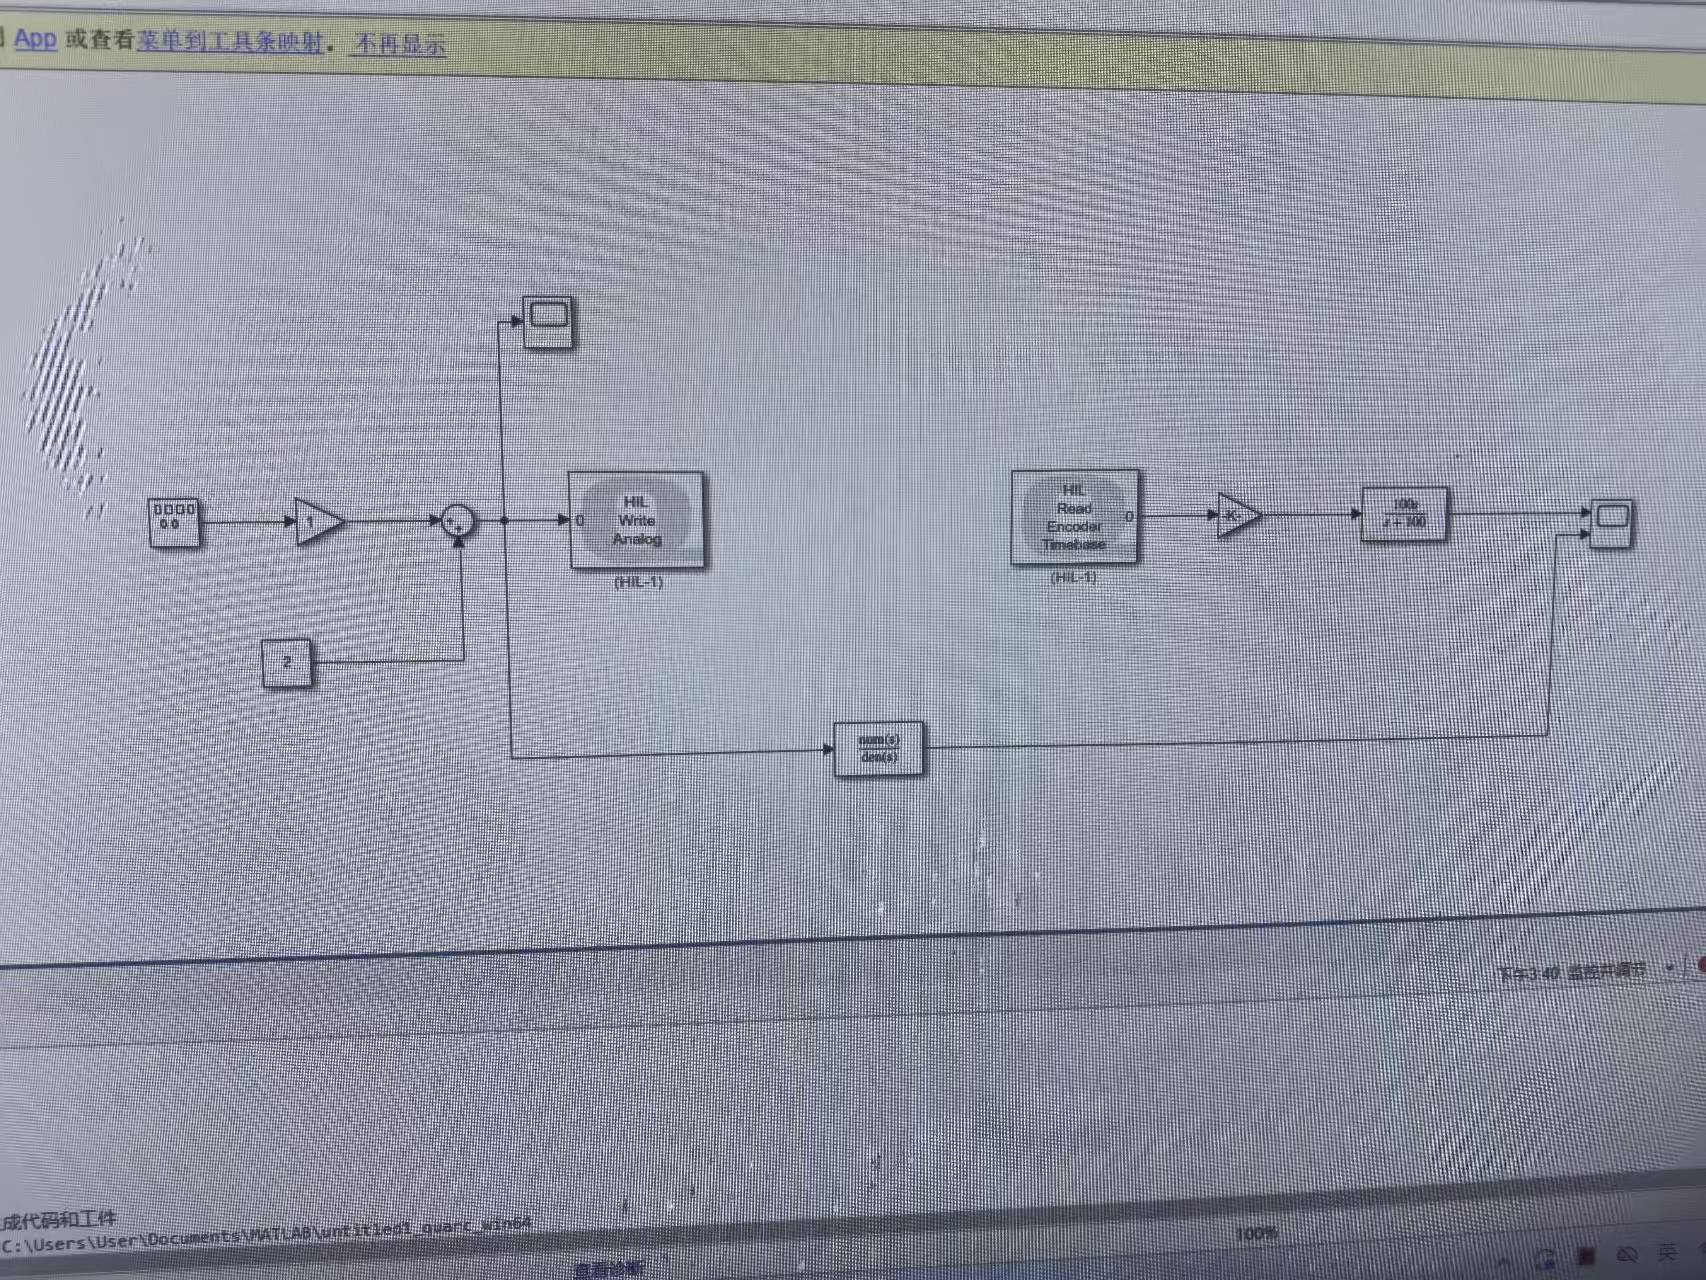
\includegraphics[width=0.98\textwidth,trim=30 170 30 230,clip]{figs/control_experiment_1/motor_model.jpg}
\caption{一阶电机模型与硬件对比结构}
\label{fig:motor_model}
\end{figure}


\subsection{位置阶跃响应对比}
将理论位置闭环与实际电机闭环置于同一Simulink模型，施加$1\unit{rad}$阶跃参考。记录驱动信号及位置响应，并读取稳态值、峰值和误差带进入时间。单位增益时驱动电压与位置误差数值相同。

\subsection{改变增益}
分别改变仿真支路和硬件支路的比例增益，比较不同阻尼工况。位置示波器比较参考位置、实际位置和仿真位置。对仿真响应与硬件响应分别计算性能指标，硬件未进入目标位置误差带时不记作完成跟踪。

\section{实验结果}
\subsection{电机转速响应}

\begin{figure}[H]
\centering
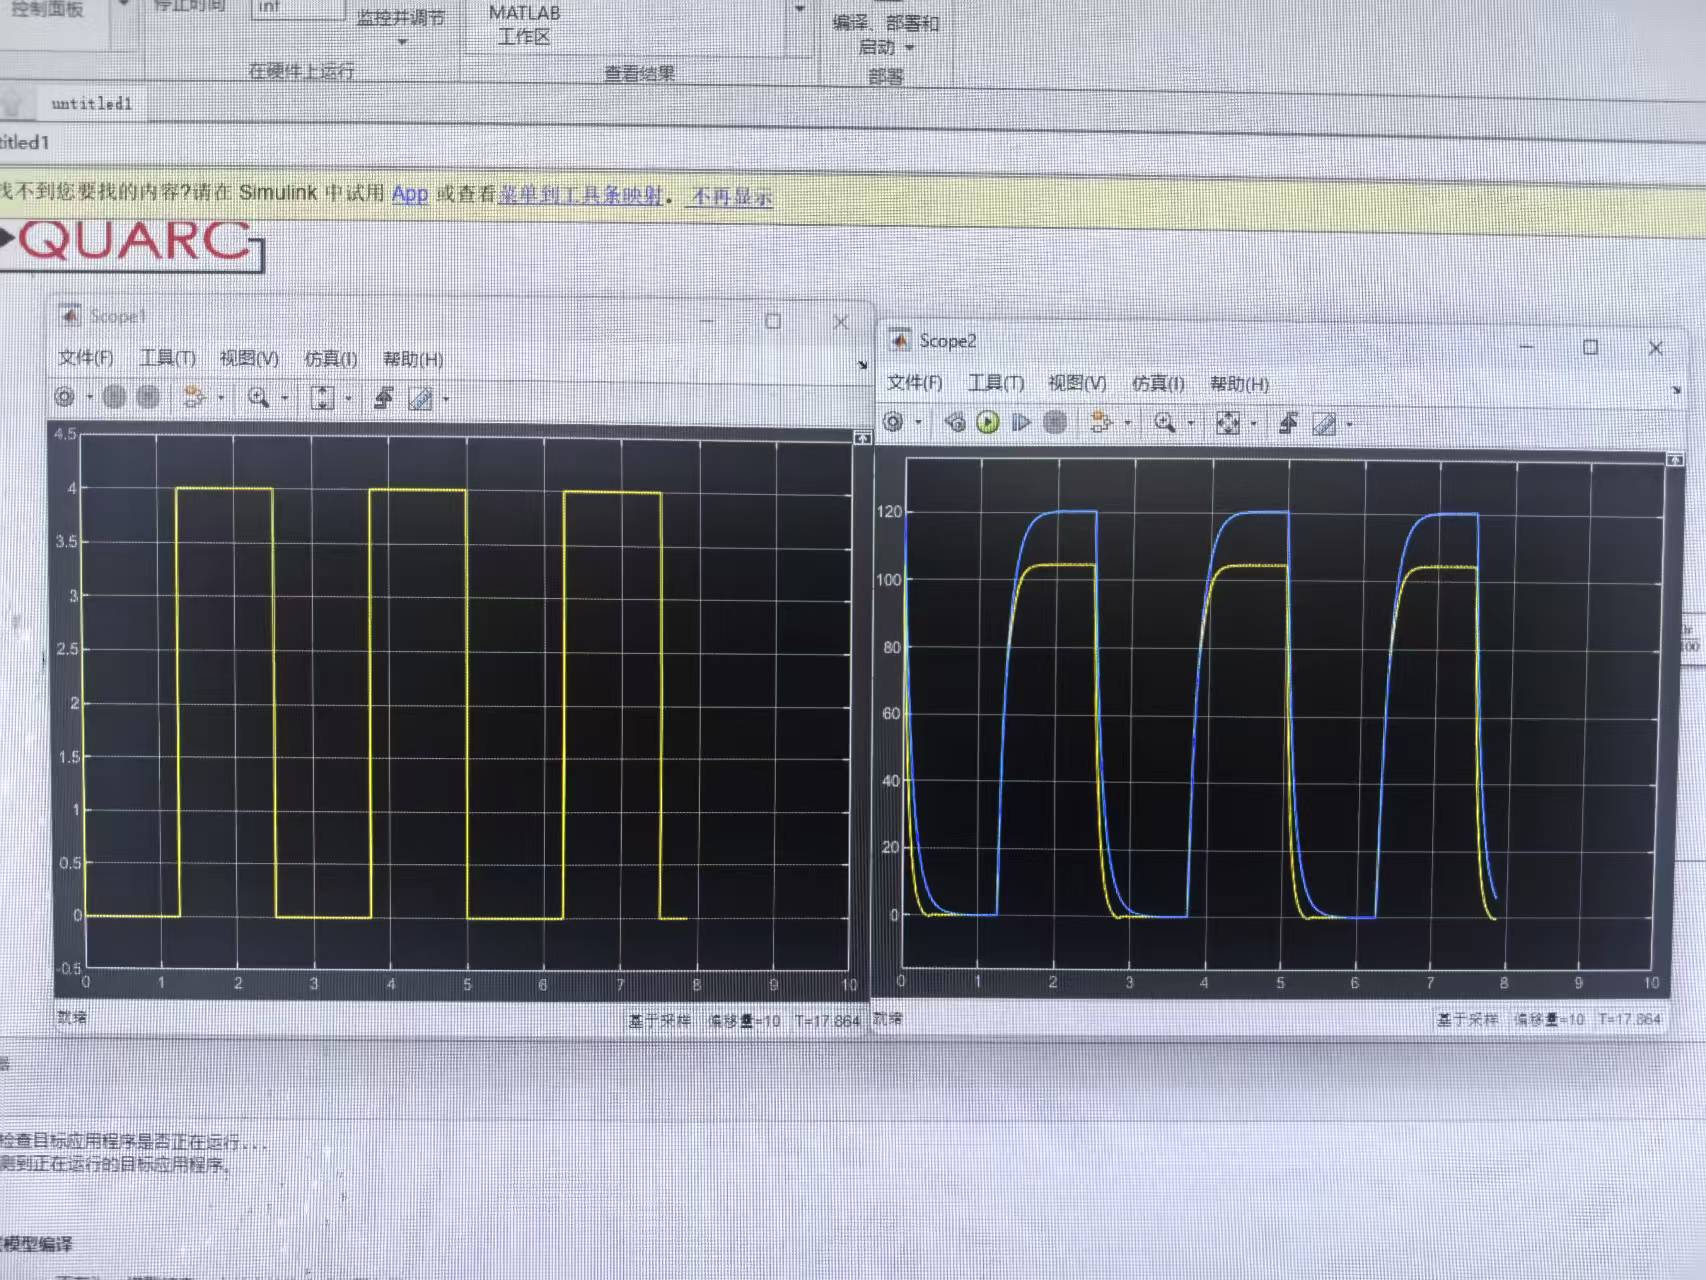
\includegraphics[width=0.98\textwidth,trim=10 150 10 230,clip]{figs/control_experiment_1/motor_square_response.jpg}
\caption{方波电压输入及转速响应}
\label{fig:motor_square_response}
\end{figure}
方波输入下，两条转速曲线均表现出惯性上升和下降，平台约为120和104。以较高平台为基准，其相对差异为
\begin{equation}
 \delta=\frac{120-104}{120}\times100\%\approx13.3\%.
\end{equation}
原始记录未保留两条转速曲线的图例，故该值仅作为平台差异，不指定理论与实测的对应颜色。

电压平台约为$4\unit{V}$，而标称模型对应的稳态转速为
\begin{equation}
 \omega_\infty=23.8095\times4\approx95.24\unit{rad/s}.
\end{equation}
标称计算值与记录平台不一致，表明需进一步校核实际使用的传递函数参数及速度换算比例。转速变化趋势与一阶惯性模型一致，但现有数据不支持认定标称模型的稳态幅值已得到验证。

\subsection{单位增益位置响应}
由式\eqref{eq:parameters}，$k_1=1$时有
\begin{equation}
 T=0.06465\unit{s},\qquad \xi=0.32485.
\end{equation}
理论超调量约$33.99\%$，$2\%$调节时间近似为$0.796\unit{s}$。


\begin{figure}[H]
\centering
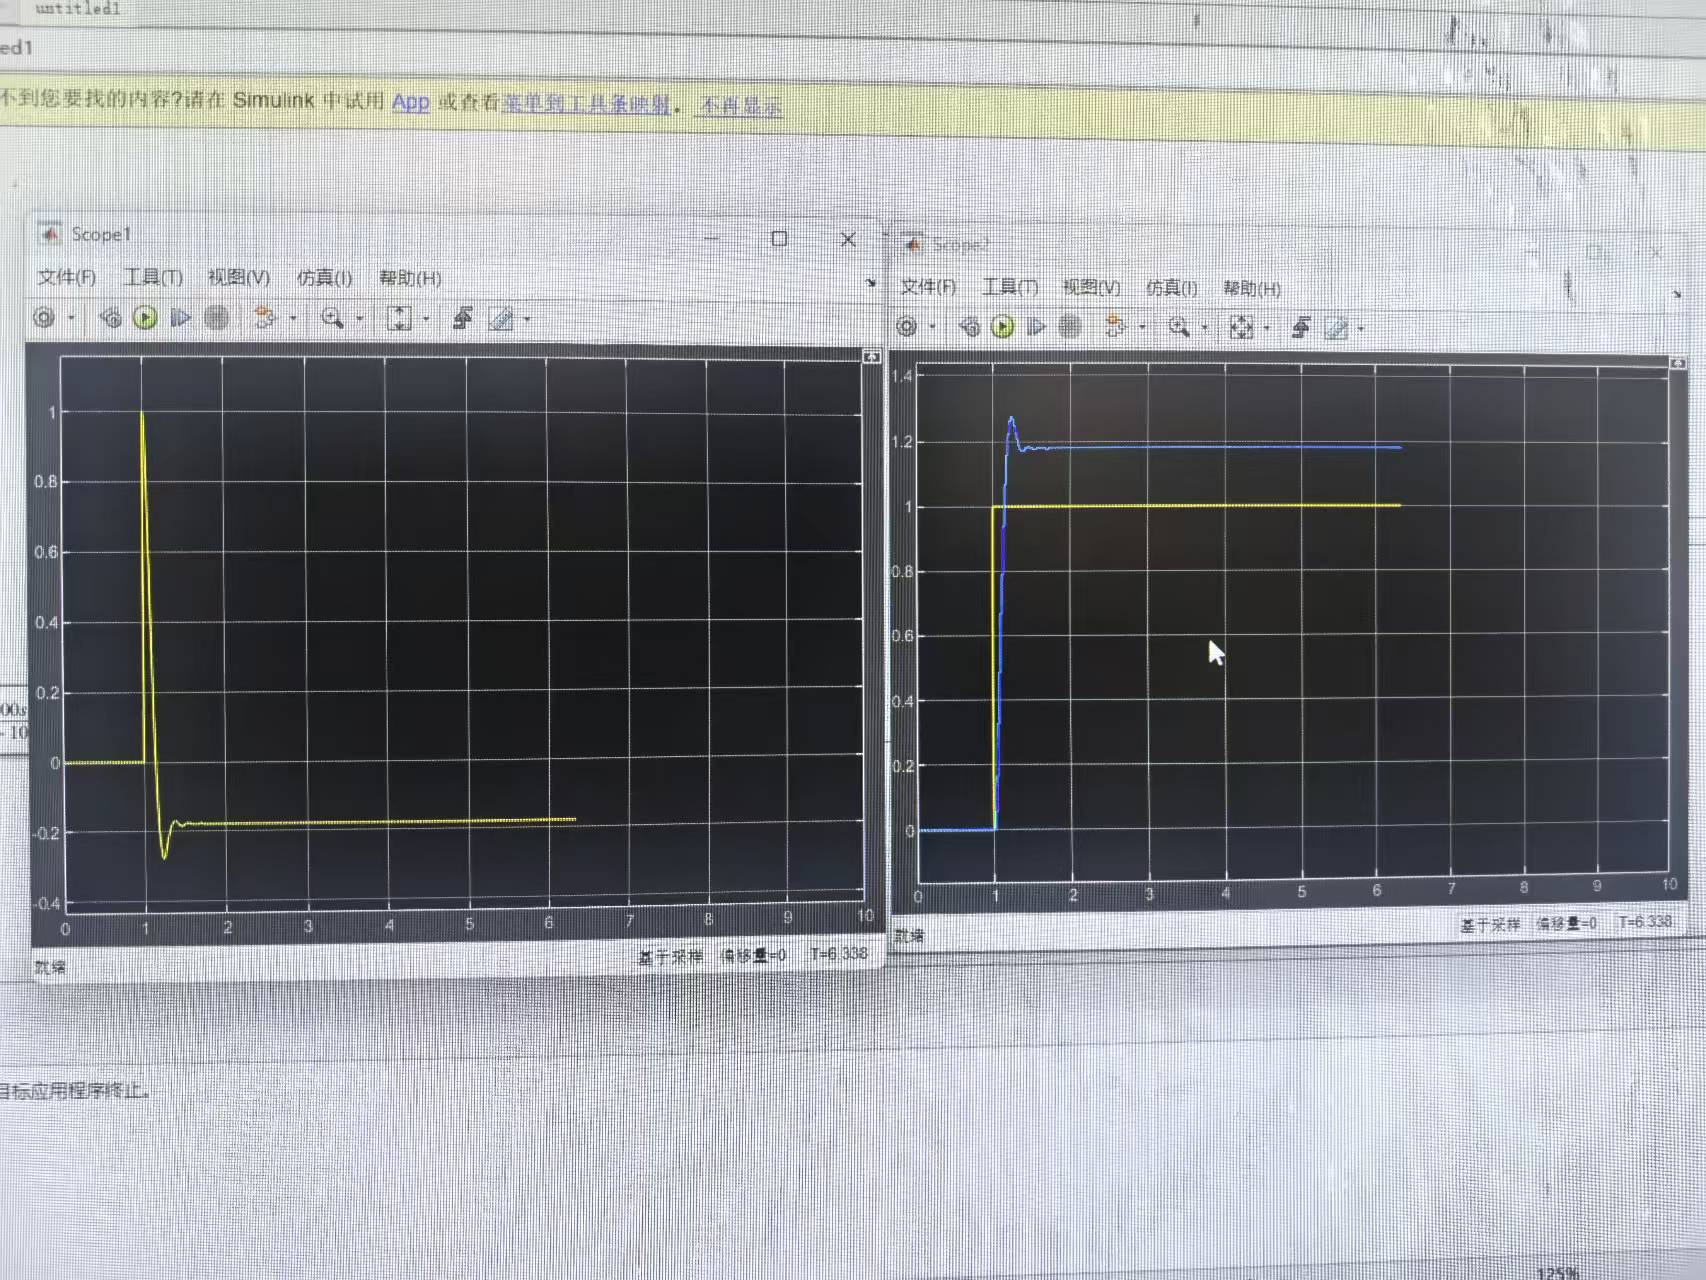
\includegraphics[width=0.98\textwidth,trim=10 230 10 190,clip]{figs/control_experiment_1/position_two_scopes.jpg}
\caption{单位增益实验的驱动信号与位置响应}
\label{fig:position_two_scopes}
\end{figure}
硬件位置响应见图\ref{fig:position_two_scopes}右侧示波器，峰值与稳态值的测量见图\ref{fig:position_peak}。稳态值为$1.158\unit{rad}$，峰值为$1.277\unit{rad}$，故
\begin{equation}
 \sigma_{\mathrm{exp}}=
 \frac{1.277-1.158}{1.158}\times100\%\approx10.3\%.
\end{equation}

\begin{figure}[H]
\centering
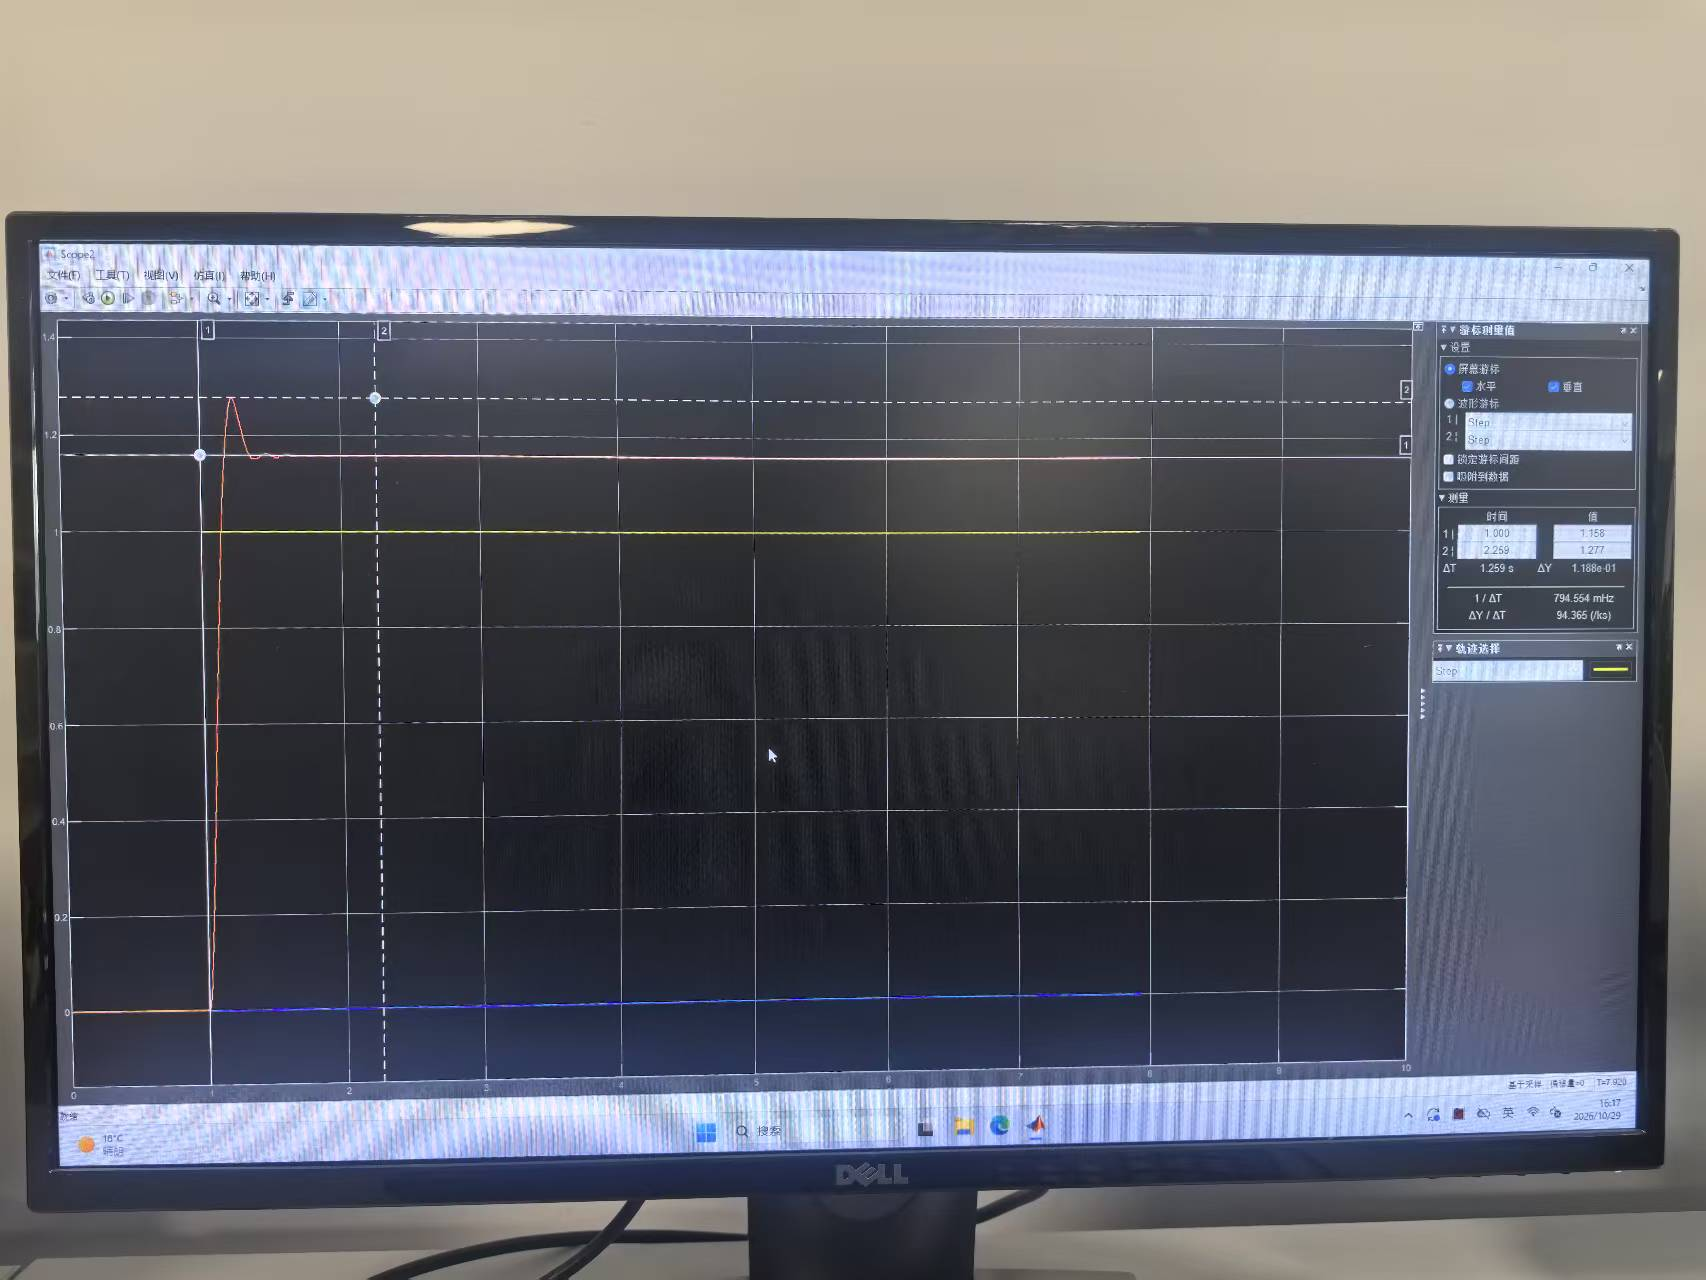
\includegraphics[width=0.98\textwidth,trim=20 100 20 175,clip]{figs/control_experiment_1/position_peak.jpg}
\caption{位置响应稳态值与峰值测量}
\label{fig:position_peak}
\end{figure}
测量中采用的误差带上下限约为1.135和$1.181\unit{rad}$，与$1.158\unit{rad}$附近的$\pm2\%$范围相符。阶跃开始于$1.000\unit{s}$，游标标记的进入时间约为$1.324\unit{s}$，得到
\begin{equation}
 t_{s,\mathrm{exp}}\approx1.324-1.000=0.324\unit{s}.
\end{equation}
该值由图\ref{fig:position_settling}中的示波器游标读出，最终越界点的判断受照片分辨率限制。
\begin{figure}[H]
\centering
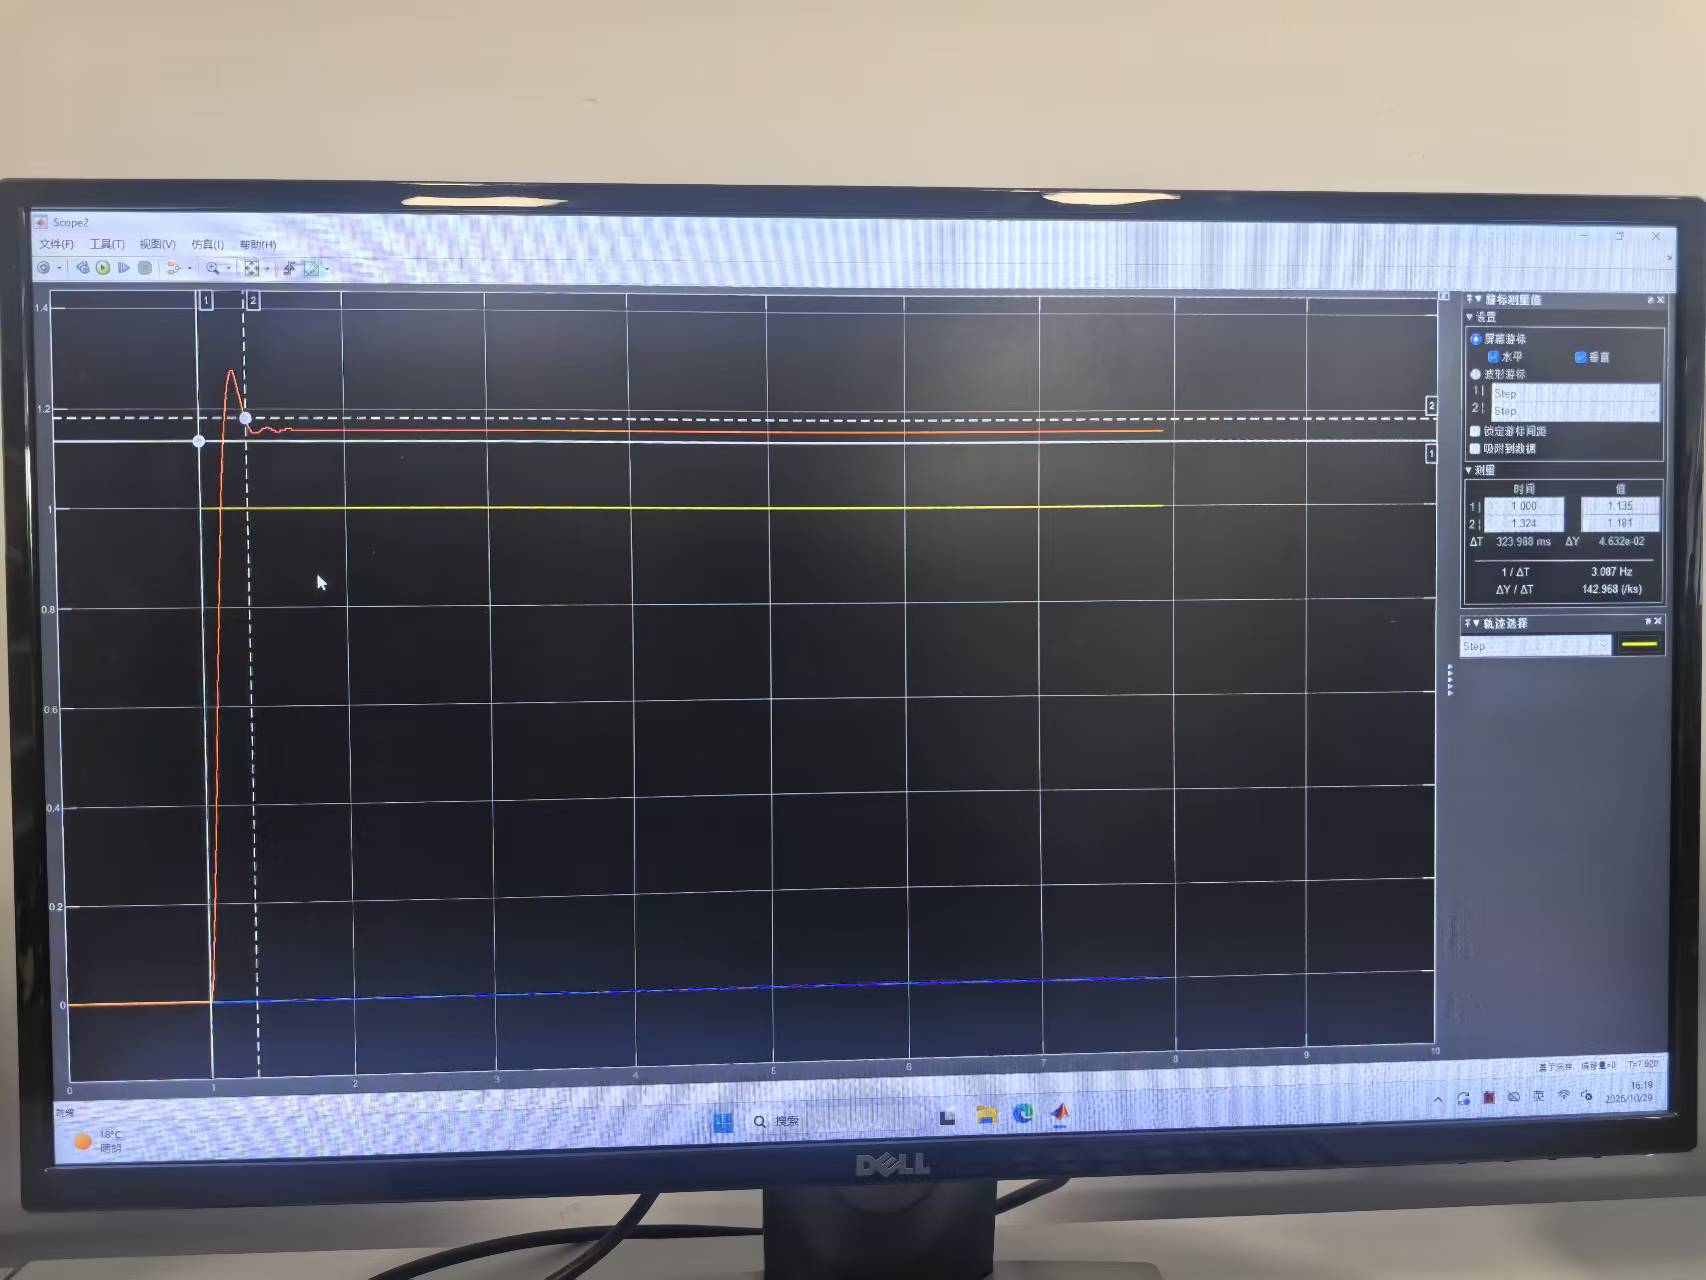
\includegraphics[width=0.98\textwidth,trim=20 100 20 175,clip]{figs/control_experiment_1/position_settling.jpg}
\caption{位置响应的2\%误差带与调节时间测量}
\label{fig:position_settling}
\end{figure}


\begin{table}[H]
\centering
\caption{单位增益位置闭环的理论与实验结果}
\begin{tabular}{lcc}
\hline
指标 & 标称理论模型 & 硬件实验\\
\hline
稳态转角/$\mathrm{rad}$ & 1 & 1.158\\
超调量/$\%$ & 33.99 & 10.3\\
$2\%$调节时间/$\mathrm{s}$ & 0.796 & 0.324\\
稳态误差/$\mathrm{rad}$ & 0 & $-0.158$\\
\hline
\end{tabular}
\label{tab:hardware}
\end{table}

驱动信号在阶跃后趋近$-0.16$，与位置误差
\begin{equation}
 e_\infty=1-1.158=-0.158\unit{rad}
\end{equation}
在数值上相符。实测位置终值偏离参考，不能将该响应视为理想单位静态增益模型的完全复现。

\subsection{不同增益下的阶跃响应}
分别取$k_1=0.08$、$0.1055$和$0.5$。本组示波器中，黄线为参考输入，蓝线为理论模型的仿真输出，红线为实际电机输出。同一增益下移动游标得到的多张照片用于读取不同指标，不作为不同实验工况。

\paragraph{理论参数。}
由$K=23.8095$、$\tau=0.0995\unit{s}$及式\eqref{eq:parameters}，得到表\ref{tab:gain_parameters}。三组分别满足$\xi>1$、$\xi\simeq1$和$0<\xi<1$。$k_1=0.1055$是临界增益的四舍五入值，因此计算所得阻尼比略大于1。

\begin{table}[H]
\centering
\caption{三组增益对应的闭环系统参数}
\begin{tabular}{lccc}
\hline
工况 & $k_1$ & $T/\mathrm{s}$ & $\xi$\\
\hline
过阻尼 & 0.08 & 0.22856 & 1.14852\\
临界阻尼附近 & 0.1055 & 0.19903 & 1.00013\\
欠阻尼 & 0.5 & 0.09142 & 0.45941\\
\hline
\end{tabular}
\label{tab:gain_parameters}
\end{table}

理论调节时间由标准二阶阶跃响应最后进入$2\%$误差带的时刻求得。过阻尼响应可写成
\begin{equation}
 y(t)=1+\frac{p_2e^{p_1t}-p_1e^{p_2t}}{p_1-p_2},\qquad
 p_{1,2}=\frac{-1\pm\sqrt{1-4\tau k_1K}}{2\tau}.
\end{equation}
数值求解$y(t_s)=0.98$，得到前两组调节时间1.695和$1.161\unit{s}$。严格临界阻尼时，
\begin{equation}
 y(t)=1-\left(1+\frac{t}{T_c}\right)e^{-t/T_c},\qquad
 T_c=2\tau,
\end{equation}
对应$t_s=5.83392T_c=1.16095\unit{s}$。
欠阻尼响应为
\begin{equation}
 y(t)=1-e^{-\xi\omega_nt}
 \left[\cos(\omega_dt)+\frac{\xi}{\sqrt{1-\xi^2}}\sin(\omega_dt)\right],
 \quad \omega_d=\omega_n\sqrt{1-\xi^2}.
\end{equation}
计算其最后一次与$0.98$或1.02相交的时刻，得到$k_1=0.5$组的理论调节时间$0.760\unit{s}$。指导书近似式$4T/\xi$给出$0.796\unit{s}$，两者的差别来自近似计算。

\paragraph{过阻尼组。}
$k_1=0.08$时，蓝色仿真输出单调上升，无超调。阶跃开始于$1.000\unit{s}$，在$2.677\unit{s}$达到0.98，仿真读图调节时间为$1.677\unit{s}$，与解析值相差$1.06\%$。红色实际输出在记录范围内接近零，没有形成趋向$1\unit{rad}$的有效响应。该组不能从实测曲线验证过阻尼动态过程。

\begin{figure}[H]
\centering
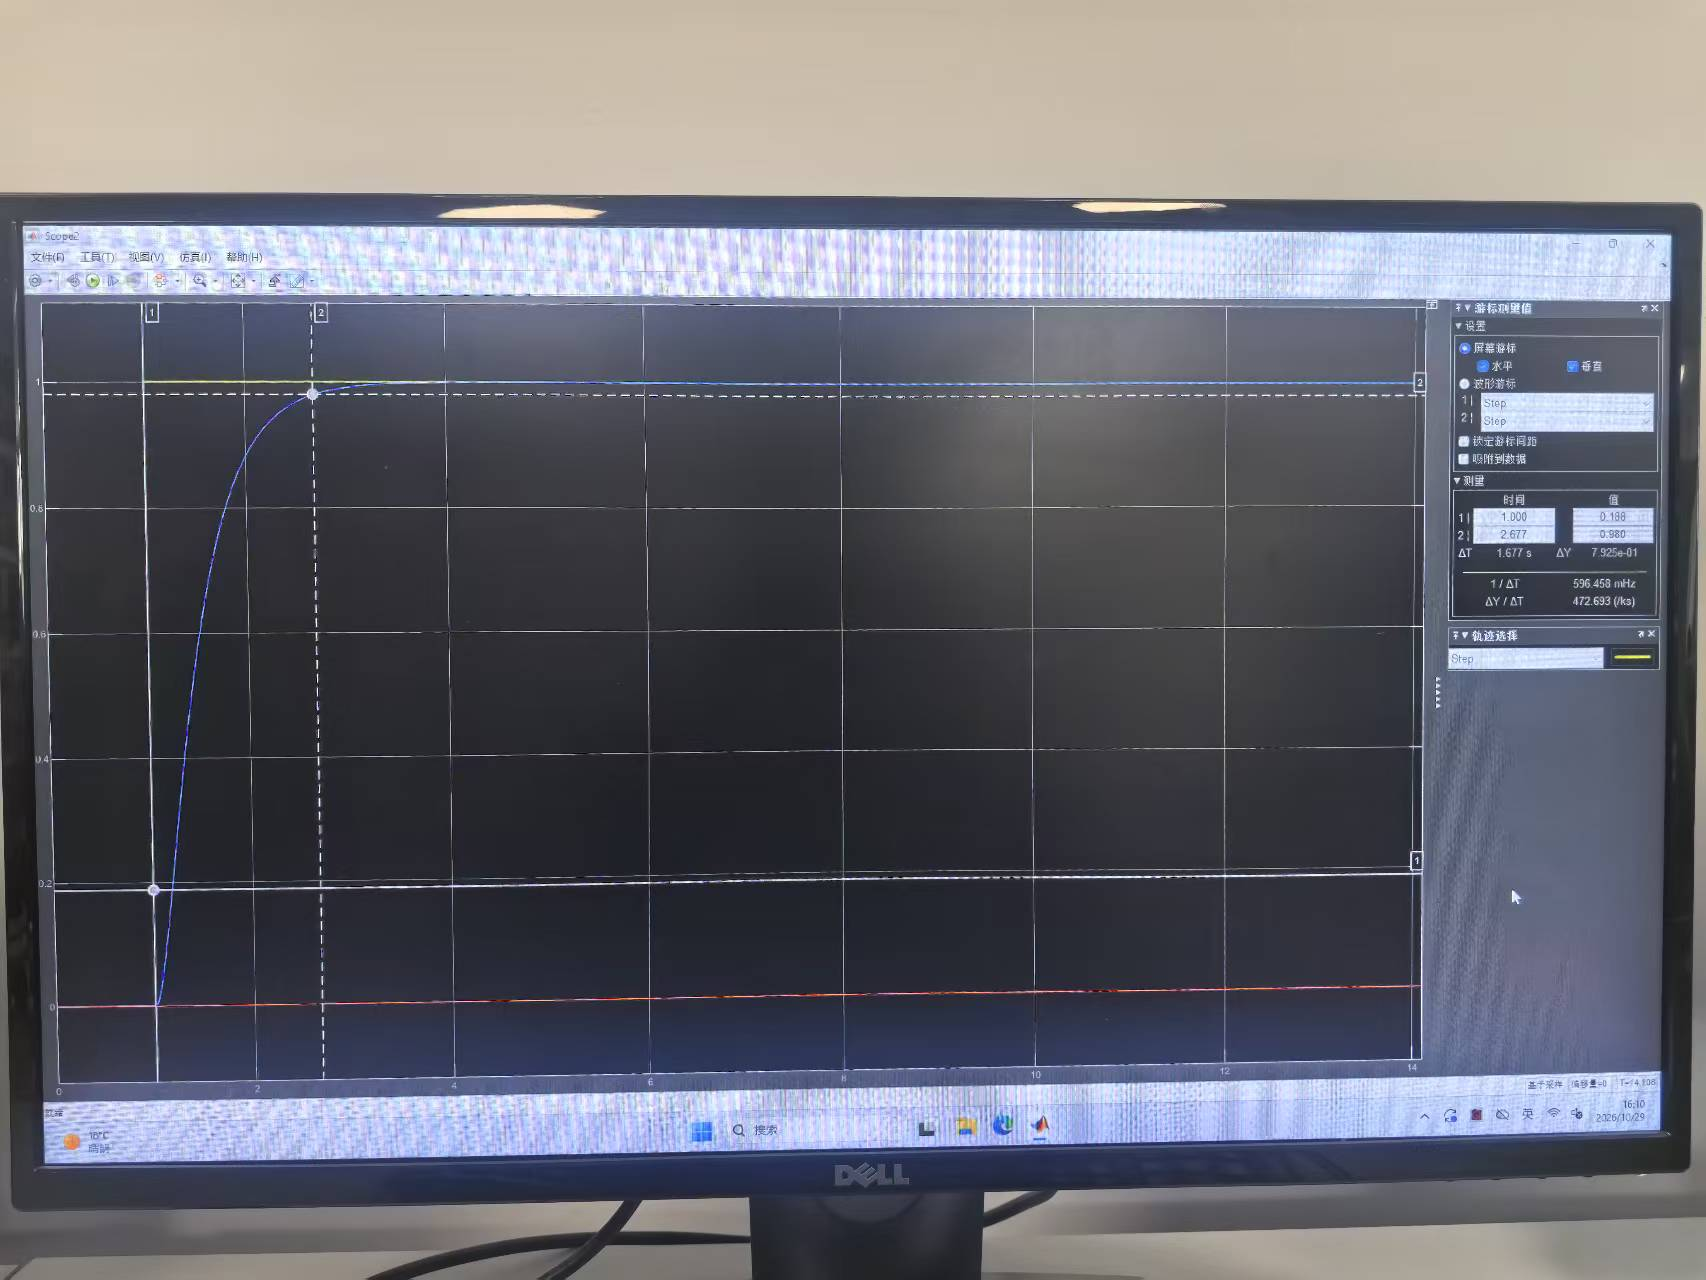
\includegraphics[width=0.98\textwidth,trim=20 100 20 175,clip]{figs/control_experiment_1/overdamped.jpg}
\caption{过阻尼组，$k_1=0.08$：蓝线为理论仿真，红线为实际输出}
\label{fig:overdamped}
\end{figure}

\paragraph{临界阻尼组。}
$k_1=0.1055$时，蓝线单调趋于1，无明显超调。游标给出的调节时间为
\begin{equation}
 t_{s,\mathrm{sim}}=2.165-1.000=1.165\unit{s},
\end{equation}
与解析值$1.16140\unit{s}$相差$0.31\%$。红线仍接近零，未获得可用于测量临界阻尼硬件响应的有效过渡过程。

\begin{figure}[H]
\centering
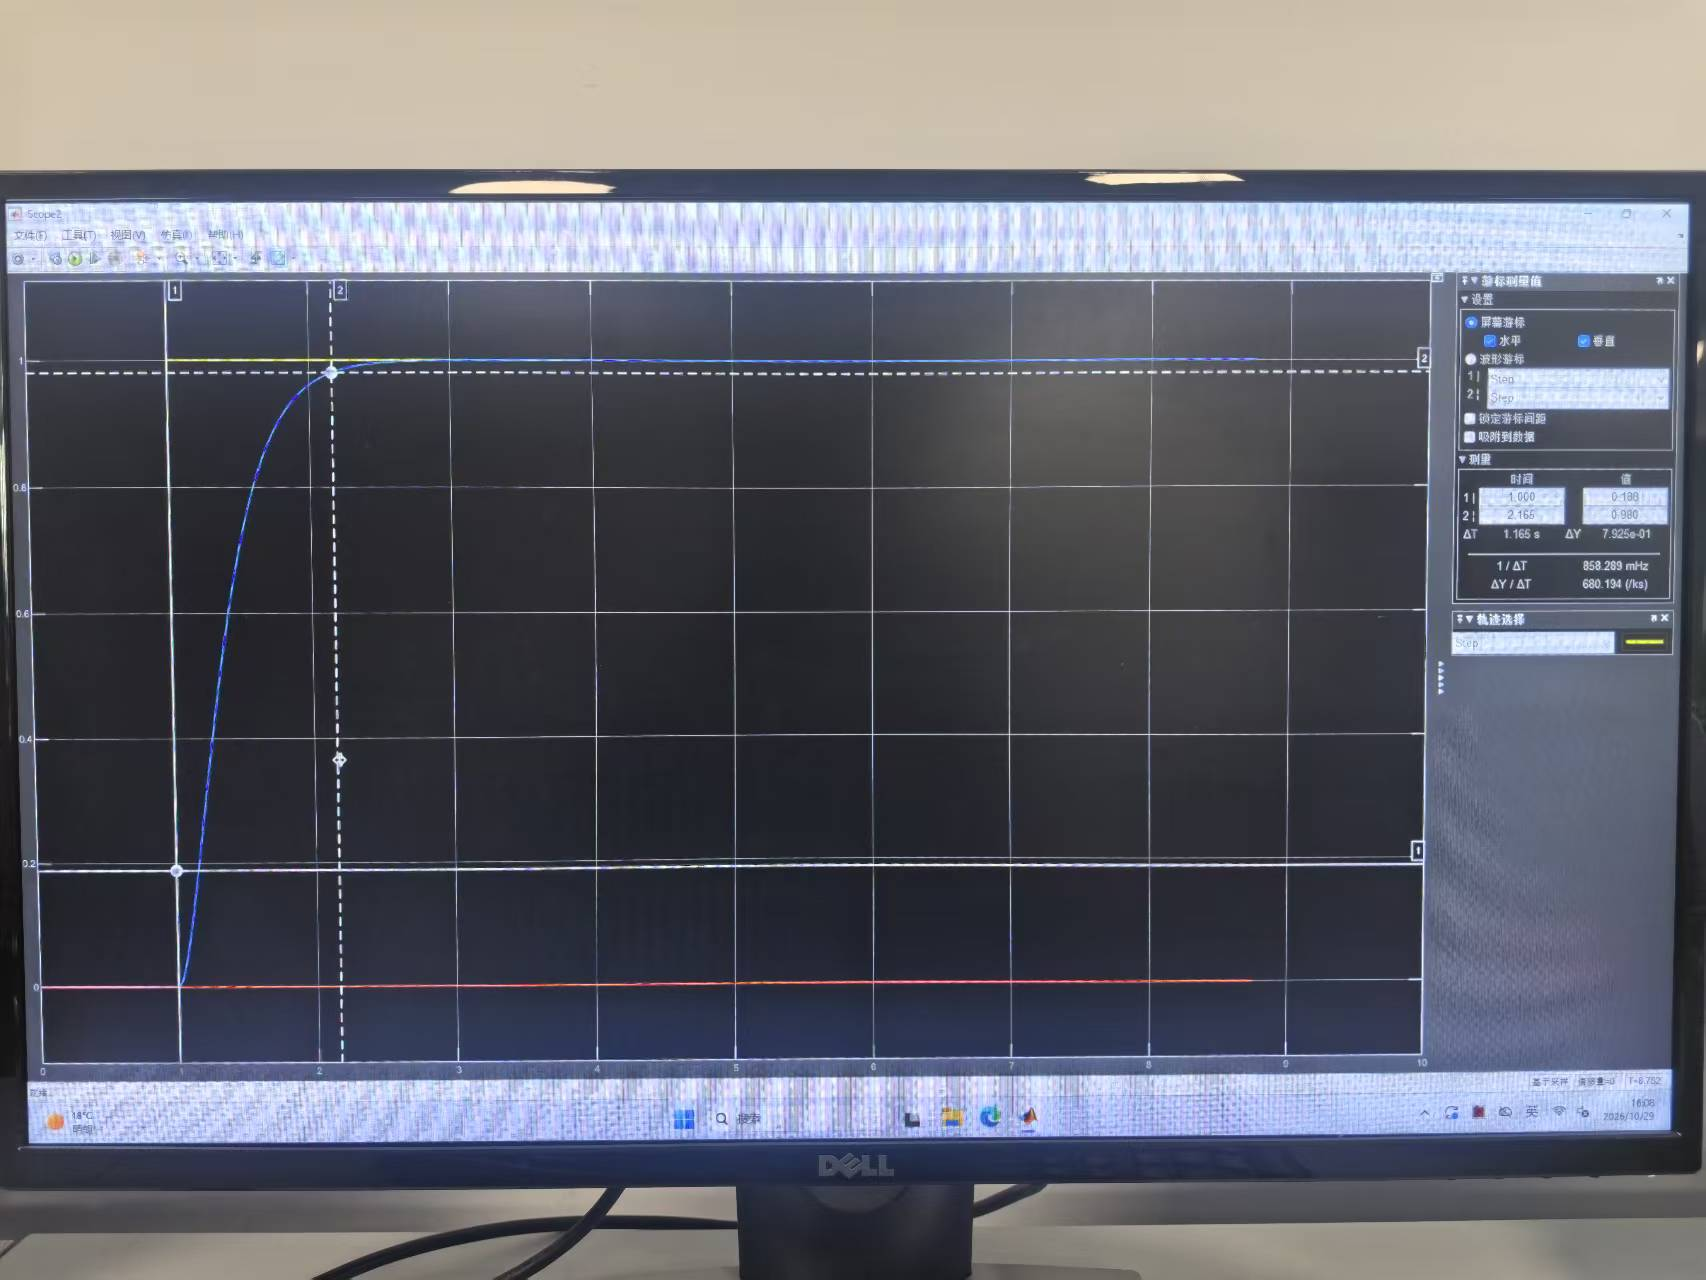
\includegraphics[width=0.98\textwidth,trim=20 100 20 175,clip]{figs/control_experiment_1/critical.jpg}
\caption{临界阻尼附近组，$k_1=0.1055$}
\label{fig:critical}
\end{figure}

\paragraph{欠阻尼组。}
$k_1=0.5$时，理论阻尼比为0.45941，解析超调量为$19.69\%$。蓝线峰值为1.198，稳态值为1，因此仿真超调量为$19.8\%$。同一工况的另一张照片用0.98与1.02标记误差带，读得
\begin{equation}
 t_{s,\mathrm{sim}}=1.767-1.000=0.767\unit{s}.
\end{equation}
其与解析调节时间$0.76026\unit{s}$相差$0.89\%$，仿真与解析计算基本一致。峰值测量图的水平游标用于读取幅值，不将其竖直游标间距作为峰值时间或调节时间。

\begin{figure}[H]
\centering
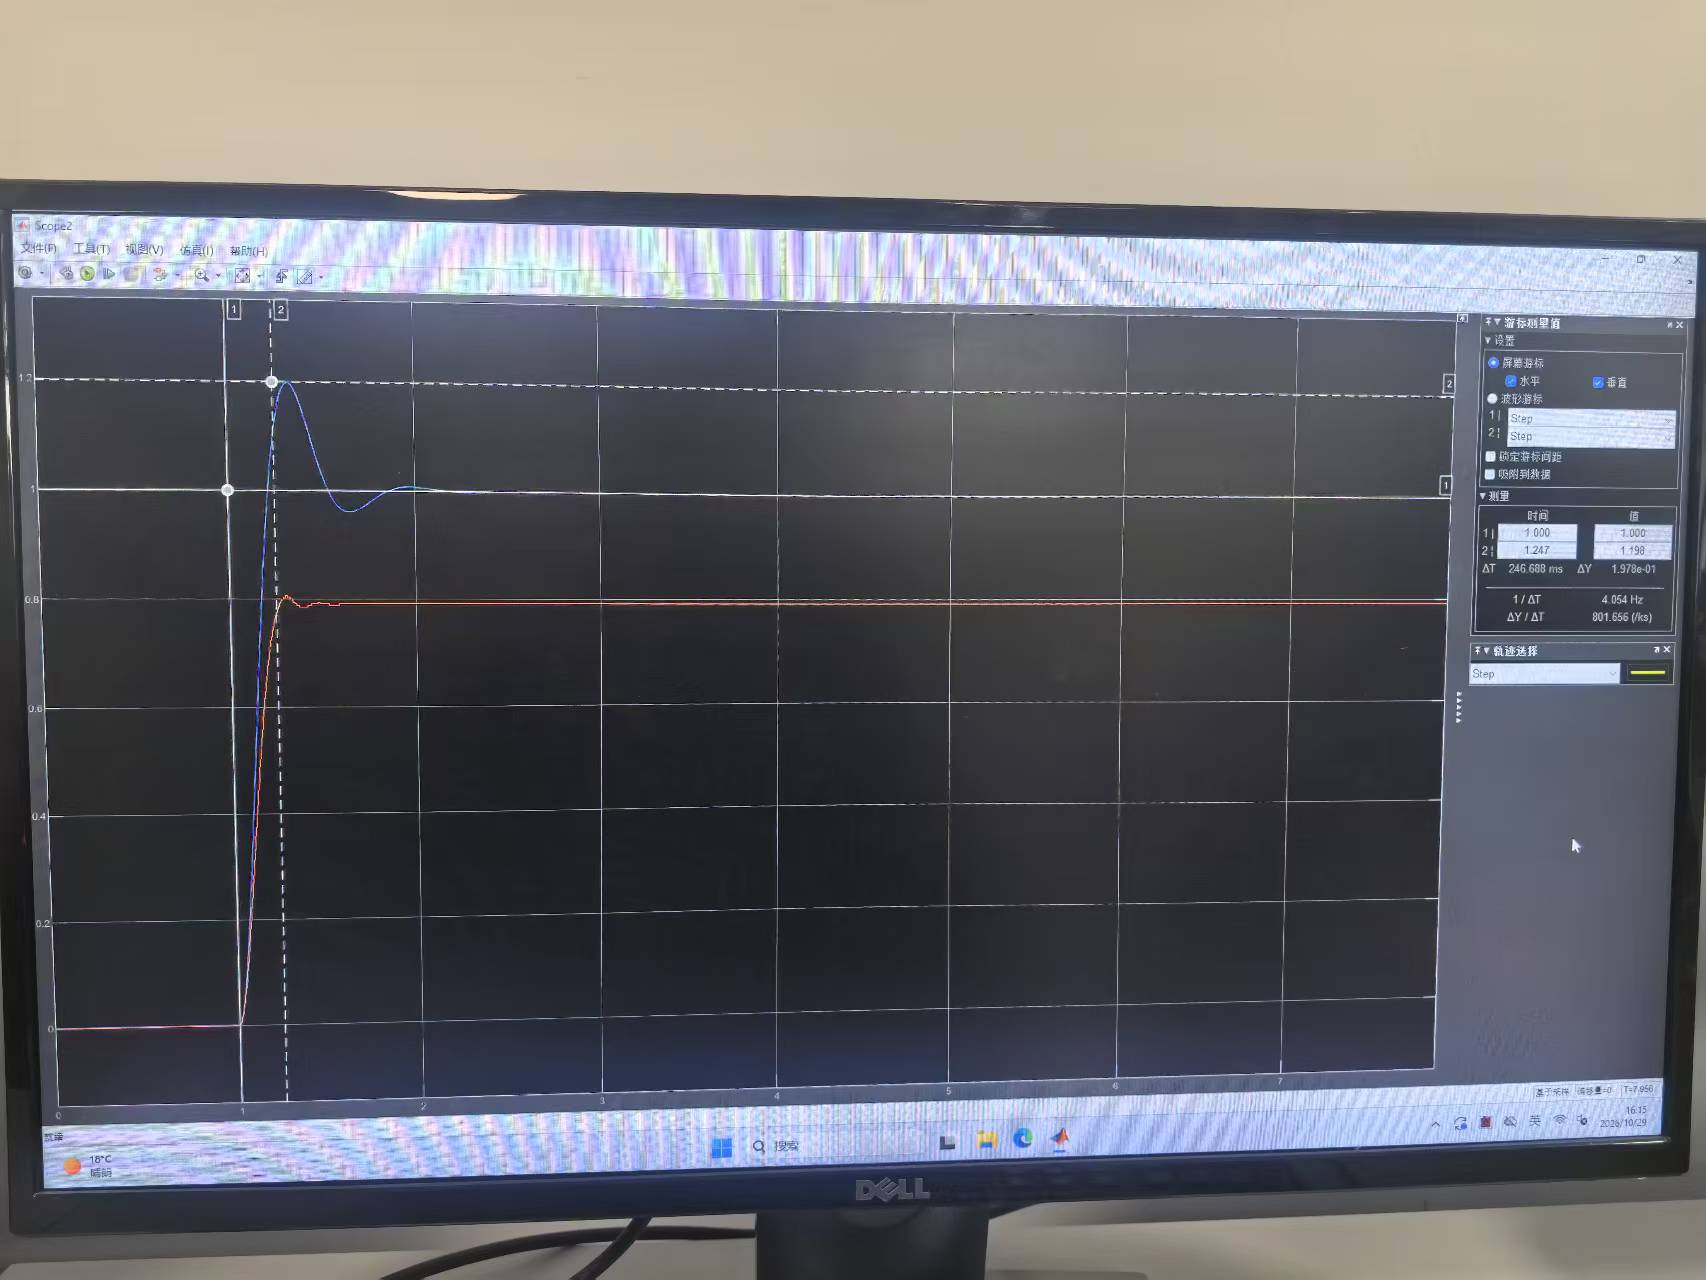
\includegraphics[width=0.98\textwidth,trim=20 100 20 175,clip]{figs/control_experiment_1/underdamped_peak.jpg}
\caption{欠阻尼组，$k_1=0.5$：蓝色仿真输出的峰值测量}
\label{fig:underdamped_peak}
\end{figure}

\begin{figure}[H]
\centering
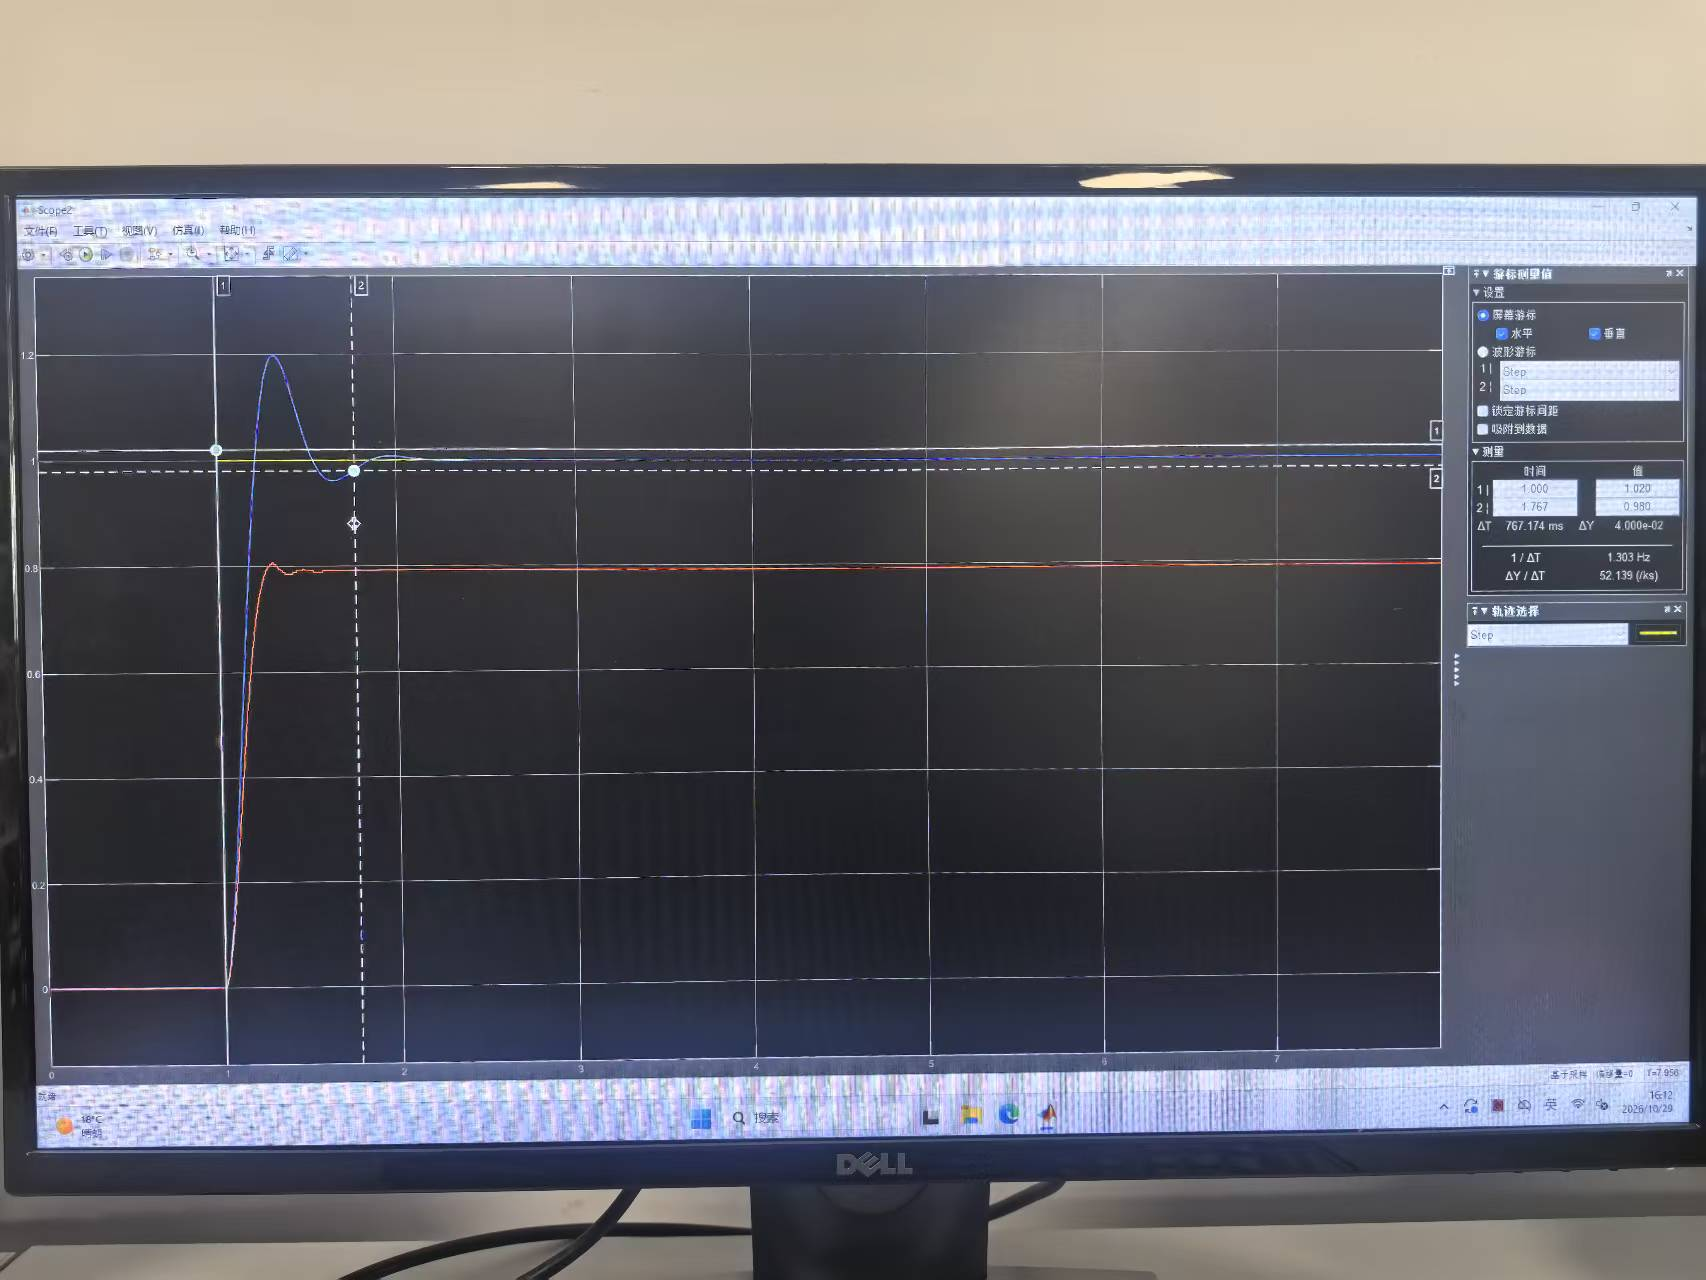
\includegraphics[width=0.98\textwidth,trim=20 100 20 175,clip]{figs/control_experiment_1/underdamped_settling.jpg}
\caption{同一欠阻尼工况下蓝色仿真输出的$2\%$调节时间测量}
\label{fig:underdamped_settling}
\end{figure}

红色实际输出的稳态值为$0.792\unit{rad}$，峰值为$0.809\unit{rad}$，实测超调量为
\begin{equation}
 \sigma_{\mathrm{exp}}
 =\frac{0.809-0.792}{0.792}\times100\%=2.15\%.
\end{equation}
稳态误差为
\begin{equation}
 e_\infty=1-0.792=0.208\unit{rad}.
\end{equation}
实测$2\%$调节时间应围绕实际终值建立误差带，即$[0.77616,0.80784]\unit{rad}$。上限与峰值仅相差$0.00116\unit{rad}$，在照片中不足一个纵向像素；峰值附近又有游标标记遮挡，不能可靠确定最后越界时刻。因此，本组不报告实测调节时间数值，也不使用蓝线的$0.767\unit{s}$代替。

\begin{figure}[H]
\centering
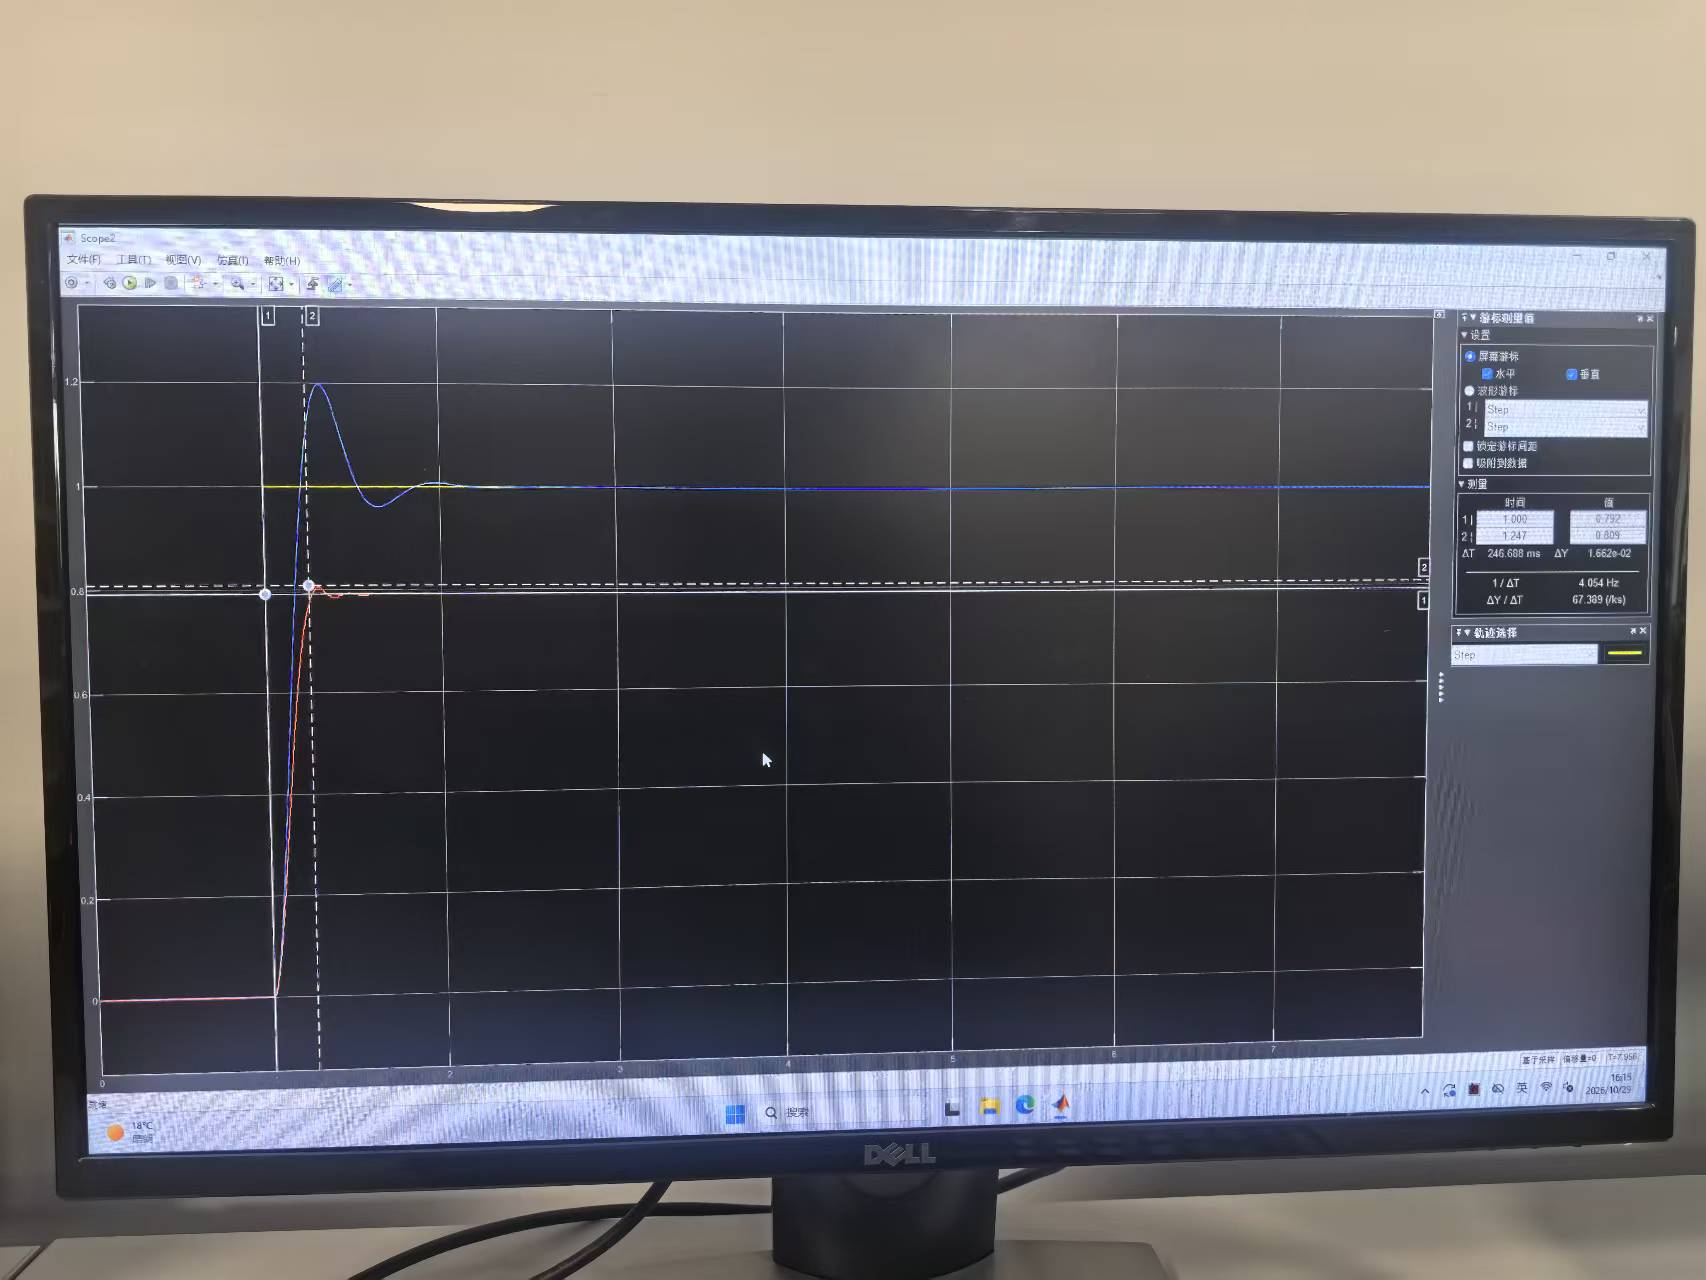
\includegraphics[width=0.98\textwidth,trim=20 100 20 175,clip]{figs/control_experiment_1/underdamped_hardware_peak.jpg}
\caption{同一欠阻尼工况下红色实际输出的稳态值与峰值测量}
\label{fig:underdamped_hardware_peak}
\end{figure}

\paragraph{理论与实测对比。}
三组结果汇总于表\ref{tab:gain_comparison}。解析理论、蓝线仿真读数和红线硬件实测分别列出。硬件无有效响应时不计算相对超调量；调节时间无法由照片可靠读取时不填数值。

\begin{table}[H]
\centering
\caption{不同增益下解析理论、仿真与硬件实测结果}
\small
\begin{tabular}{ccccccc}
\hline
 & \multicolumn{2}{c}{解析理论} & \multicolumn{2}{c}{理论仿真（蓝线）} & \multicolumn{2}{c}{硬件实测（红线）}\\
$k_1$ & $\sigma/\%$ & $t_s/\mathrm{s}$ & $\sigma/\%$ & $t_s/\mathrm{s}$ & $\sigma/\%$ & $t_s/\mathrm{s}$\\
\hline
0.08 & 0 & 1.695 & 0 & 1.677 & --- & 无有效响应\\
0.1055 & 0 & 1.161 & 0 & 1.165 & --- & 无有效响应\\
0.5 & 19.69 & 0.760 & 19.8 & 0.767 & 2.15 & 未准确读取\\
\hline
\end{tabular}
\label{tab:gain_comparison}
\end{table}

欠阻尼组实测超调量比解析理论值低17.54个百分点，但同时存在$0.208\unit{rad}$稳态误差，不能仅由超调较小判断硬件性能更好。三组理论模型均有$\Phi(0)=1$，而实际输出未准确到达目标，说明标称线性模型不足以解释全部实验现象。实际硬件三种阻尼状态的完整定量验证尚未由本组记录实现。

\section{分析与讨论}
\subsection{时间常数与阻尼比对阶跃响应的影响}
在阻尼比固定时，减小$T$会增大自然频率，压缩响应时间尺度，而超调量保持不变；在$T$固定时，减小$\xi$会增强振荡并增大超调。过阻尼响应无超调，但过大的阻尼使响应变慢；临界阻尼响应单调，较过阻尼组更快；欠阻尼响应出现超调及衰减振荡。

本实验通过增益同时改变$T$与$\xi$。由$k_1=0.08$增大至0.5，$T$由$0.22856\unit{s}$减小至$0.09142\unit{s}$，$\xi$由1.14852减小至0.45941。蓝线仿真由单调上升变为振荡响应，超调量由0增至$19.8\%$，调节时间由$1.677\unit{s}$减至$0.767\unit{s}$，与上述理论变化一致。这些变化由理论仿真得到，不能直接作为硬件已实现同样动态变化的证据。

在本模型中，
\begin{equation}
 \frac{T}{\xi}=2\tau.
\end{equation}
故在指导书近似公式适用的欠阻尼范围内，$t_s\approx4T/\xi=8\tau$。提高增益并不意味着调节时间持续减小，实际调节时间还受振荡相位及最后越界位置影响。

\subsection{理论与实测差异}
两组低增益记录中的零输出，指实际转角在照片分辨率内接近$0\unit{rad}$，不是超调量为0或调节时间为0。比例控制电压为
\begin{equation}
 u=k_1(r-\theta).
\end{equation}
初始位置为零、参考为$1\unit{rad}$时，$k_1=0.08$和0.1055分别只产生$0.08\unit{V}$和$0.1055\unit{V}$的初始驱动。低速时忽略电感压降及反电动势，以$R_m=8.4\,\Omega$、$k_t=0.042\unit{N\cdot m/A}$估计电磁转矩：
\begin{equation}
 M_m\simeq\frac{k_t}{R_m}u
 =\begin{cases}
 0.400\unit{mN\cdot m},&k_1=0.08,\\
 0.528\unit{mN\cdot m},&k_1=0.1055.
 \end{cases}
\end{equation}
这两个工况只能提供很小的起动转矩。实际电机具有静摩擦及驱动死区，小电压可能不足以使电机起动。电机保持静止后，误差仍为$1\unit{rad}$；比例控制没有积分积累作用，驱动电压保持不变，不能自行提高到起动阈值。因此会出现蓝色理想模型响应正常上升，而红色实际转角保持接近零的现象。

这一解释也与$k_1=0.5$组存在稳态误差相符：电机停止在$0.792\unit{rad}$时，按控制律得到残余驱动电压$u=0.5(1-0.792)=0.104\unit{V}$，与低增益组的驱动电压处于同一量级。该数值由控制律计算，不是额外测得的电压。本次未测起动电压及摩擦转矩，故静摩擦和死区是与数据相符的物理解释，尚不能排除驱动链路异常；应通过电压逐级增加试验及HIL输出检查加以区分。

欠阻尼组红线稳态值低于参考，实际振荡也弱于模型。摩擦和未建模阻尼会影响衰减特性，设备参数、编码器换算及反馈偏置也可能造成差异。单位增益组输出高于参考，而$k_1=0.5$组输出低于参考，因此应同时检查反馈比例、偏置和模型设置，不能将全部偏差归因于摩擦。

\subsection{测量限制与实验改进}
硬件定量验证需要在三组增益下分别保存实际位置原始时间序列，校准反馈比例与零点，并检查电机的起动电压。对低增益工况应先排查驱动与采集链路，再判断线性二阶模型是否适用。欠阻尼硬件调节时间应由原始采样数据按实际终值的$2\%$误差带求取，避免用照片中接近像素分辨率的差别确定最后越界时刻。

\section{思考题}
\subsection{思考题1：改变截止频率对滤波结果的影响}
一阶低通滤波器为
\begin{equation}
 G_f(s)=\frac{\omega_f}{s+\omega_f},\qquad
 |G_f(\mathrm j\omega)|=\frac{\omega_f}{\sqrt{\omega^2+\omega_f^2}}.
\end{equation}
将截止频率由$10\unit{rad/s}$增大至$200\unit{rad/s}$时，滤波器时间常数$1/\omega_f$由$0.1\unit{s}$减小至$0.005\unit{s}$。截止频率降低，高频噪声衰减增强，转速曲线更平滑，但响应滞后增大，快速变化被削弱；截止频率提高，滤波响应更快，保留的动态细节增多，同时微分噪声也更明显。因此，应在噪声抑制和动态响应之间折中选择截止频率。

\subsection{思考题2：由超调量和调节时间求系统参数}
在已知比例增益$k_1$且响应可由标准欠阻尼二阶模型描述时，可以估计$K$与$\tau$。设超调比例$M_p=\sigma/100$，先由超调量求阻尼比：
\begin{equation}
 \xi=\frac{-\ln M_p}{\sqrt{\pi^2+(\ln M_p)^2}}.
\end{equation}
再利用$2\%$调节时间近似式及本系统的参数关系，得到
\begin{equation}
 t_s\approx\frac{4T}{\xi}=8\tau,\qquad
 \tau\approx\frac{t_s}{8},\qquad
 K\approx\frac{1}{4k_1\tau\xi^2}.
\end{equation}
以$k_1=0.5$组的仿真读数$M_p=0.198$、$t_s=0.767\unit{s}$为例，得到$\xi\approx0.458$、$\tau\approx0.0959\unit{s}$，进而求得$K\approx24.84$，与标称参数$\tau=0.0995\unit{s}$、$K=23.8095$接近。差异来自调节时间近似公式及读图误差。若采用$5\%$调节时间，则相应有$\tau\approx t_s/6$。

该方法要求模型适用且增益已知。明显存在死区或静摩擦的低增益硬件响应不宜直接套用；临界阻尼及过阻尼组无超调，也不能仅靠超调量确定阻尼比。

\section{实验结论}
一阶模型能够描述电机转速的主要惯性特征，但记录平台与标称模型存在差异，需要校核参数及速度换算。单位增益位置实验中，实际响应的超调量约为$10.3\%$，相对实际稳态值的$2\%$调节时间约为$0.324\unit{s}$，稳态位置误差约为$-0.158\unit{rad}$。

$k_1=0.08$、0.1055和0.5分别对应过阻尼、临界阻尼附近和欠阻尼理论参数。三组蓝线仿真的调节时间为1.677、1.165和$0.767\unit{s}$，与解析计算一致。红色硬件输出在两组低增益下未形成有效响应；欠阻尼组实测超调量为$2.15\%$、稳态误差为$0.208\unit{rad}$，调节时间未能可靠读取。因此，理论三种阻尼状态得到仿真验证，但硬件三种阻尼状态的完整定量验证仍存在缺项，需结合驱动检查与原始采样补充实验。


\end{document}
